\documentclass[11pt]{article}

% Packages
\usepackage{graphicx}   % for pictures
\usepackage{amsthm}     % for math
\usepackage{amsmath, mathtools}    %   more math
\usepackage{amsfonts}   %   more math
\usepackage{physics}    % more symbols
\usepackage{circuitikz} % for circuit diagrams
\usepackage{amssymb}    % math symbols
\usepackage{siunitx}    % units
\usepackage{mathrsfs}   % fancy text
\usepackage{color}      % colored letters for notes and reminders
\usepackage{float}      % for image location

%The amsthm package lets you format different types of mathematical ideas nicely. You use it by defining "\newtheorem"s as below:
\newtheorem{problem}{Problem}
\newtheorem{theorem}{Theorem}
\newtheorem*{proposition}{Proposition}
\newtheorem{lemma}[theorem]{Lemma}
\newtheorem{corollary}[theorem]{Corollary}
\theoremstyle{definition}
\newtheorem{defn}[theorem]{Definition}

% Magins

\setlength{\voffset}{0.1in}
\setlength{\paperwidth}{8.5in}
\setlength{\paperheight}{11in}
\setlength{\headheight}{14pt}
\setlength{\headsep}{0.5in}
\setlength{\textheight}{11in}
\setlength{\textheight}{8in}
\setlength{\topmargin}{-0.25in}
\setlength{\textwidth}{7in}
\setlength{\topskip}{0in}
\setlength{\oddsidemargin}{-0.25in}
\setlength{\evensidemargin}{-0.25in}

% For images in this document:
\graphicspath{ {images/} }

% User Defined Commands
\newcommand{\nder}[2]{\frac{d^{#1} #2}{d t^{#1}}}   % The nth derivative wrt t: {n}{x(t)}
\newcommand{\der}[1]{\frac{d #1}{d t}}              % Derivative wrt t: {x(t)}
\newcommand{\infint}{\int_{-\infty}^{\infty}}       % Integral from - infinity to + infinity
\newcommand{\infsum}[1]{\sum_{#1 = -\infty}^{\infty}}% Sum of a variable from - to + infinity
\newcommand{\para}[1]{\left( #1 \right)}            % Instead of writing parenthesis all the time

% User Command for Wider Matrices
\makeatletter
\renewcommand*\env@matrix[1][\arraystretch]{%
  \edef\arraystretch{#1}%
  \hskip -\arraycolsep
  \let\@ifnextchar\new@ifnextchar
  \array{*\c@MaxMatrixCols c}}
\makeatother


% Heading:
\usepackage{fancyhdr}
\pagestyle{fancy}
\lhead{Nicholas Pham}
\chead{ES 155}          %   Change the Class!!
\rhead{Homework 8}   %   Change the Problem Set Number!!


% ----- BEGIN DOCUMENT-----
\begin{document}

\textbf{\huge{ES 155 Homework 8}}    %   Change the Class and Problem Set Number!!
\normalsize

Please see attached MATLAB code for computations throughout.

\begin{enumerate}

    \item % Problem 1
    In this problem, the controller should stabilize the system with requirements:
    \begin{itemize}
        \item Steady State error $<$ 1\%
        \item Phase Margin $>$ $30^o$
    \end{itemize}
    In addition, the bandwidth is defined as the maximum frequency at which the closed loop system can track the input with less than 25\% error.  In general, the method used to design the controller is to attempt to compute a reasonable value for the parameters, then use MATLAB's $\mathtt{controlSystemDesigner()}$ to check.

    \begin{enumerate}
        \item % 1.a
        A disk drive read head positioning system might have a plant transfer function

        $$ P(s) = \frac{1}{s^3 + 10s^2 + 3s + 10} $$

        To reach a steady state error of less than 1\%, the set the closed loop transfer function for the error at $s = 0$ to be less that 0.01:

        \begin{align*}
            H_{e\rightarrow r} = E(s) &= \frac{1}{1+L(s)} \\
            E(0) &= \frac{1}{1+L(0)} < 0.01 \\
        \end{align*}

        assuming a large $L(0)$, this means that

        $$ L(0) > 100 \quad\quad (+40 \text{ dB}) $$

        Because $L(s) = P(s)C(s)$ and $P(0) = 0.1$ or -20 dB, controller needs to add at least +60 dB of gain at steady state.  For some safety margin, set $k_p = 3162.3$ or +70 dB.  With the controller transfer function $C(s) = 3162.3$, the phase margin was $-53^o$, which did not meet the requirement.  To improve this, I added a zero at 1 rad/s.  The resulting phase margin was $9.14^o$, still shy of the goal.  Adjusting the frequency could only result in at best a $12^o$ phase margin at 3.5 rad/s, so achieving the requirements in with this method utilizing only a single zero with no integrator is infeasible.

        As an alternative approach, an integrator was used to reduce the steady state error to zero.  Introducing a single zero at 1 rad/s was sufficient to reach a $94^o$ phase margin, satisfying both requirements.

        This system controller is given by

        $$ C(s) = \frac{s + 1}{s} $$

        Computing the bandwidth as tracking to 25\% error, requires 

        $$ T(s) = \frac{L(s)}{1 + L(s)} < 0.25 $$ 

        so

        $$ L(s) + 1 > 4 $$

        up to the bandwidth.  This can be computed via MATLAB's $\mathtt{bandwidth(sys, dbdrop)}$ function, where $\mathtt{dbdrop}$ is the allowable error, in this case 25\% or -12.0 dB.  The bandwidth for this system is 1.2651 rad/s.

        \item % 1.b
        A drug administration model might have a system plant transfer function 

        $$ P(s) = \frac{1.5s + 0.75}{s^2 + 0.7s + 0.05} $$

        Using a similar method to the disk drive positioning system, the open loop transfer function $L(s)$ should have a +40 dB gain at steady state.  In this case,$P(0) = 15$ or +23.5 dB, so $C(s)$ needs to add only +20 dB at $s = 0$.  The resulting phase margin for

        $$ C(s) = 10 $$

        is $90.8^o$ , so this controller satisfies both requirements.  In this case, the steady state error is 0.66\%, while the 25\% error bandwidth is 58.46 rad/s.

    \end{enumerate}

    \item % Problem 2
    For a vectored thrust aircraft with system plant transfer function

    $$ P(s) = \frac{r}{Js^2 + cs + mgl}$$

    where $g, l, m, J, c, r$ are given constants, a controller is required to achieve

    \begin{itemize}
        \item Steady state error $<$ 2\%
        \item Tracing error $<$ 10\% from 0 to 1 rad/s
        \item Phase margin $>$ $40^o$
    \end{itemize}

    \begin{enumerate}
        \item % 2.a
        To begin, the open loop Bode plot is plotted in Figure \ref{fig:2.a}, annotated with the desired constraints.  In particular, the Magnitude plot includes a rectangle in the upper left corner.  The steady state (zero frequency) gain should be above the upper edge of the rectangle, and the magnitude should remain over the lower edge until the right edge, at 1 rad/s.  The Phase plot shows the requirement for the phase margin, where the vertical line is the zero gain crossing point and the horizontal line is $-180^o$ plus the desired $40^o$ phase margin.  The phase plot should cross the vertical line above the horizontal one.

        \begin{figure}[H]
            \centering
            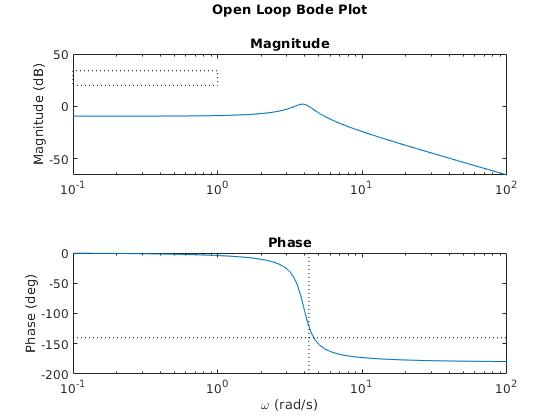
\includegraphics[width = 0.8\textwidth]{ES155P8_2a.jpg}
            \caption{Open Loop Bode plot of vectored thrust aircraft.  The dotted lines indicate the desired constraints.}
            \label{fig:2.a}
        \end{figure}

        \item % 2.b
        As above, to achieve a 2\% or better steady state error, $L(0) > 1/0.02 = 50$ or +34 dB.  $P(0) = 0.3401$ or -9.37 dB.  This means the controller needs to add 43.4 dB gain.  To ensure success, try +50dB, or 316.28.  The tracing error specification requires

        $$ T(s) = \frac{L(s)}{1 + L(s)} < 0.1 \quad \forall \quad s \in [0,1]$$

        or $L(s) > 10$ (+20 dB).  The Bode plot from the $\mathtt{controlSystemDesigner()}$ shows that this is satisfied.  However, the phase margin for this setup is only $1.48^o$.  Adding a zero at 1 rad/s increases the phase margin to $90^o$ while maintaining the other requirements. The resulting open loop Bode plot for the system with control

        $$ C(s) = 316.2 (s + 1) $$

        is shown in Figure \ref{fig:2b}

        \begin{figure}[H]
            \centering
            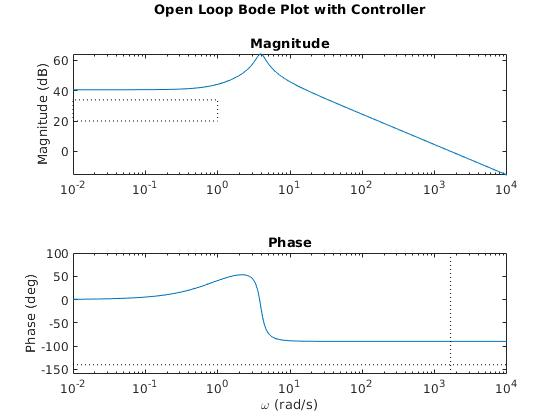
\includegraphics[width = 0.8\textwidth]{ES155P8_2b.jpg}
            \caption{Open Loop Bode plot with controller.  The dotted lines indicate the desired constraints as above: they are now satisfied.}
            \label{fig:2b}
        \end{figure}

        Examining the closed loop system also shows that the design requirements are satisfied.  Using MATLAB, the steady state error is 0.92\%, the 10\% bandwidth is $1.67 \times 10^4$ rad/s, and the phase margin is $90^o$.

        \item % 2.c

        Figure \ref{fig:2c} shows the step and frequency response for the closed loop system.

        \begin{figure}[H]
            \centering
            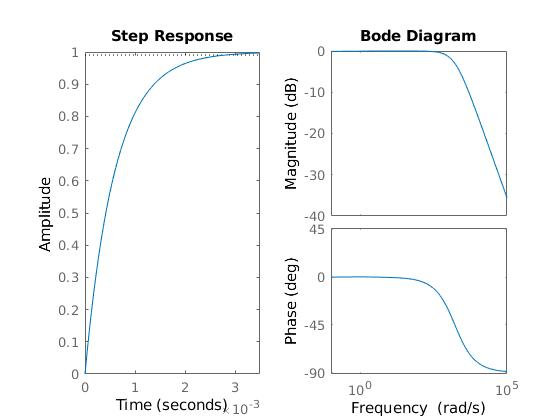
\includegraphics[width = 0.8\textwidth]{ES155P8_2c.jpg}
            \caption{Closed loop step and frequency response.}
            \label{fig:2c}
        \end{figure}

        $\mathtt{stepinfo()}$ gives that the rise time is 0.0013 s, the overshoot is 0.818, and the settling time is 0.0021 s.  The steady state error, compute by subtracting the system's DC gain from 1 is 0.0092.


    \end{enumerate}

    \item % Problem 3
    A magnetic levitation system with transfer function 

    $$ P(s) = \frac{k}{s^2 - r^2} $$

    must be stabilized.

    \begin{enumerate}
        \item % 3.a
        The plant transfer function has two poles, making it unstable.  To stabilize the system, add a zero at 1 rad/s, making

        $$ C(s) = s + 1 $$

        With this controller, the open loop transfer function $L(s) = 4000 \frac{s + 1}{s^2 - 625}$, according to the given parameter values.  This transfer function has a zero at -1 and poles at $\pm 25$.
        On the other hand, the closed loop transfer function $4000\frac{s + 1}{s^2 + 4000s + 3375}$ has a zero at -1 and poles at -3999.2 and -0.8, indicating that the closed loop system is stable.  

        \item % 3.b
        The Nyquist plots of the open loop transfer function $L(s) = P(s)C(s)$ and the closed loop transfer function $4000\frac{s + 1}{s^2 + 4000s + 3375}$ are shown in Figure \ref{fig:3b}

        \begin{figure}[H]
            \centering
            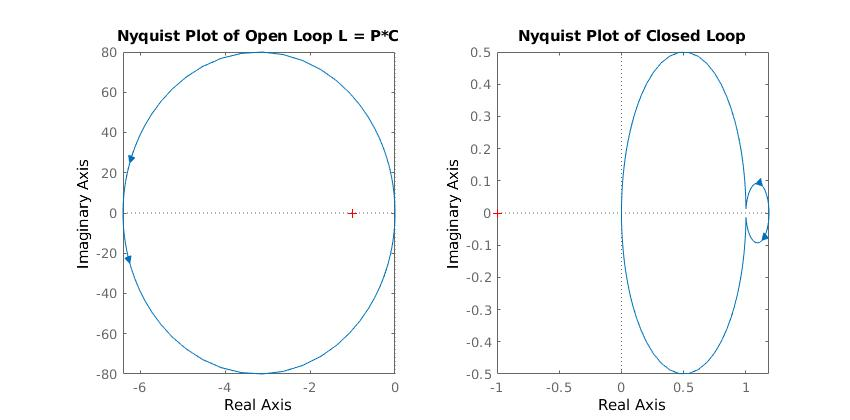
\includegraphics[width = 0.8\textwidth]{ES155P8_3b.jpg}
            \caption{Nyquist plots of open and closed loop system.}
            \label{fig:3b}
        \end{figure}

        The Nyquist Criterion states that for a system to be stable, $Z = 0$ where $Z = N + P$ and $P$ =  the number of poles in $L(s)$ in the region enclosed by the D contour and $N$ = the number of clockwise encirclements of -1 by the Nyquist plot.  In the open loop case, there is one pole enclosed by the D contour at 25, but there is a counterclockwise encirclement of -1 in the Nyquist plot, so $Z = 1-1=0$ and the open loop system is stable.  In the closed loop case, there are no poles in the region of the D-contour, and -1 is not encircled in the Nyquist plot, so $Z = 0 + 0 = 0$ and again the system is stable.

        \item % 3.c

        Figure \ref{fig:3c} shows the Bode plots for $S$ and $T$.

        \begin{figure}[H]
            \centering
            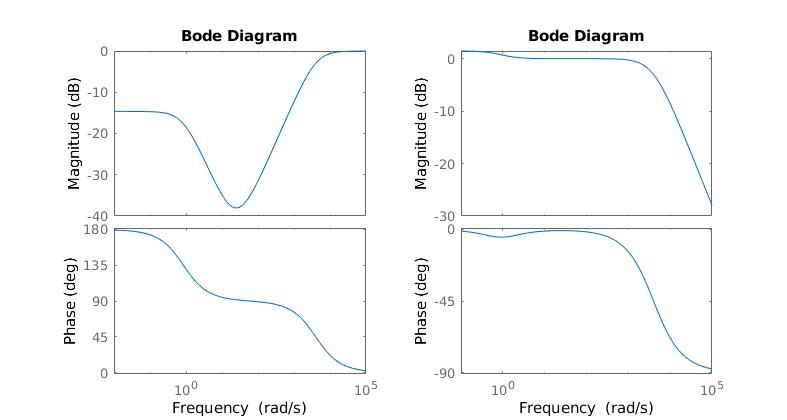
\includegraphics[width = 0.8\textwidth]{ES155P8_3c.jpg}
            \caption{Bode plot for $S = \frac{1}{1 + L}$ on the left and $T = \frac{L}{1+L}$ on the right.}
            \label{fig:3c}
        \end{figure}

    \end{enumerate}

\end{enumerate}
\end{document}


